\newpage

\hformbar

\formdesc{Méthodologie étage d'entrée}

\hformbar

\formtitle{Superposition : }

Exprimer nœuds par nœuds les potentielles 
Pour définir le gain total et les tensions de référence

\formtitle{Définition de la dynamique :}

La dynamique est la plage de tension sur laquelle il est possible de travailler.

Exemple :

$Av = 5 $

$+vcc = 10 V$

$-vcc = 0 V$

$ Dynamique_{in} = 10/5 = 2 V $ 

\formtitle{Mode Commun :}

$Gain_{reel} = Gain + erreur$

$U_{in\;MC}  = \cfrac{Uin(+) + Uin(-)}{2}$

$Uout_{MC} = \cfrac{Uout(+) + Uout(-)}{2} $  

et garder la composante AC 

\hformbar

\formtitle{Bruit de quantification : }

$SNRQ = 20log(\cfrac{Vrms}{Uref}) + 4.77 + 6.02 * N$\\

$N = \cfrac{SNRQ - 20log(\cfrac{Vrms}{Uref}) - 4.77}{6.02}$

\formtitle{Surechantillionage : }

$\Delta SNRQ = SNRQ1 - SNRQ2$\\

$Nosr = 10^{\cfrac{\Delta SNRQ}{10}}$\\



\formtitle{Filtre d'anti-repliement : }

$Pente = \cfrac{\Delta dB}{20\,log(\cfrac{f_e}{f_c})}$

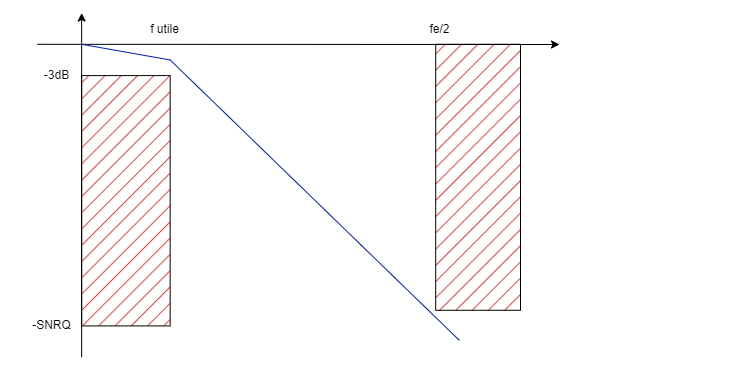
\includegraphics[width = 0.7\textwidth]{Test.drawio.png}


\hformbar


\formtitle{Convertisseur : }

Calcul par étape : 

$Uco_n = Uref \cdot \cfrac{1}{D\#(N-n-1)} - Uin$

Si Uco > 0 alors comparateur à 1 et on ne garde pas le bit $D\#n$

Exemple si $Uco_2$ Et N = 8 et étape 2 mais $D\#5$ :

Si comp = 1 : 

$Uco_3 = Uref \cdot \cfrac{1}{D\#4} - Uin$

Si comp = 0 : 

$Uco_3 = Uref \cdot (\cfrac{1}{D\#5} + \cfrac{1}{D\#4}) - Uin$